\documentclass[author-year, review, 11pt]{components/elsarticle} %review=doublespace preprint=single 5p=2 column
%%% Begin My package additions %%%%%%%%%%%%%%%%%%%
\usepackage[hyphens]{url}
\usepackage{lineno} % add 
  \linenumbers % turns line numbering on 
\bibliographystyle{elsarticle-harv}
\biboptions{sort&compress} % For natbib
\usepackage{graphicx}
\usepackage{booktabs} % book-quality tables
%% Redefines the elsarticle footer
\makeatletter
\def\ps@pprintTitle{%
 \let\@oddhead\@empty
 \let\@evenhead\@empty
 \def\@oddfoot{\it \hfill\today}%
 \let\@evenfoot\@oddfoot}
\makeatother

% A modified page layout
\textwidth 6.75in
\oddsidemargin -0.15in
\evensidemargin -0.15in
\textheight 9in
\topmargin -0.5in
%%%%%%%%%%%%%%%% end my additions to header

\usepackage[T1]{fontenc}
\usepackage{lmodern}
\usepackage{amssymb,amsmath}
\usepackage{ifxetex,ifluatex}
\usepackage{fixltx2e} % provides \textsubscript
% use upquote if available, for straight quotes in verbatim environments
\IfFileExists{upquote.sty}{\usepackage{upquote}}{}
\ifnum 0\ifxetex 1\fi\ifluatex 1\fi=0 % if pdftex
  \usepackage[utf8]{inputenc}
\else % if luatex or xelatex
  \usepackage{fontspec}
  \ifxetex
    \usepackage{xltxtra,xunicode}
  \fi
  \defaultfontfeatures{Mapping=tex-text,Scale=MatchLowercase}
  \newcommand{\euro}{€}
\fi
% use microtype if available
\IfFileExists{microtype.sty}{\usepackage{microtype}}{}
\usepackage{color}
\usepackage{fancyvrb}
\newcommand{\VerbBar}{|}
\newcommand{\VERB}{\Verb[commandchars=\\\{\}]}
\DefineVerbatimEnvironment{Highlighting}{Verbatim}{commandchars=\\\{\}}
% Add ',fontsize=\small' for more characters per line
\usepackage{framed}
\definecolor{shadecolor}{RGB}{248,248,248}
\newenvironment{Shaded}{\begin{snugshade}}{\end{snugshade}}
\newcommand{\KeywordTok}[1]{\textcolor[rgb]{0.13,0.29,0.53}{\textbf{{#1}}}}
\newcommand{\DataTypeTok}[1]{\textcolor[rgb]{0.13,0.29,0.53}{{#1}}}
\newcommand{\DecValTok}[1]{\textcolor[rgb]{0.00,0.00,0.81}{{#1}}}
\newcommand{\BaseNTok}[1]{\textcolor[rgb]{0.00,0.00,0.81}{{#1}}}
\newcommand{\FloatTok}[1]{\textcolor[rgb]{0.00,0.00,0.81}{{#1}}}
\newcommand{\CharTok}[1]{\textcolor[rgb]{0.31,0.60,0.02}{{#1}}}
\newcommand{\StringTok}[1]{\textcolor[rgb]{0.31,0.60,0.02}{{#1}}}
\newcommand{\CommentTok}[1]{\textcolor[rgb]{0.56,0.35,0.01}{\textit{{#1}}}}
\newcommand{\OtherTok}[1]{\textcolor[rgb]{0.56,0.35,0.01}{{#1}}}
\newcommand{\AlertTok}[1]{\textcolor[rgb]{0.94,0.16,0.16}{{#1}}}
\newcommand{\FunctionTok}[1]{\textcolor[rgb]{0.00,0.00,0.00}{{#1}}}
\newcommand{\RegionMarkerTok}[1]{{#1}}
\newcommand{\ErrorTok}[1]{\textbf{{#1}}}
\newcommand{\NormalTok}[1]{{#1}}
\usepackage{longtable}
\usepackage{graphicx}
% We will generate all images so they have a width \maxwidth. This means
% that they will get their normal width if they fit onto the page, but
% are scaled down if they would overflow the margins.
\makeatletter
\def\maxwidth{\ifdim\Gin@nat@width>\linewidth\linewidth
\else\Gin@nat@width\fi}
\makeatother
\let\Oldincludegraphics\includegraphics
\renewcommand{\includegraphics}[1]{\Oldincludegraphics[width=\maxwidth]{#1}}
\ifxetex
  \usepackage[setpagesize=false, % page size defined by xetex
              unicode=false, % unicode breaks when used with xetex
              xetex]{hyperref}
\else
  \usepackage[unicode=true]{hyperref}
\fi
\hypersetup{breaklinks=true,
            bookmarks=true,
            pdfauthor={},
            pdftitle={rgbif: R client for working with GBIF species occurrence data},
            colorlinks=true,
            urlcolor=blue,
            linkcolor=magenta,
            pdfborder={0 0 0}}
\urlstyle{same}  % don't use monospace font for urls
\setlength{\parindent}{0pt}
\setlength{\parskip}{6pt plus 2pt minus 1pt}
\setlength{\emergencystretch}{3em}  % prevent overfull lines
\setcounter{secnumdepth}{0}
% Pandoc toggle for numbering sections (defaults to be off)
\setcounter{secnumdepth}{0}
% Pandoc header



\begin{document}
\begin{frontmatter}

  \title{rgbif: R client for working with GBIF species occurrence data}
    \author[cstar]{Scott Chamberlain\corref{c1}}
   \ead{scott(at)ropensci.org} 
   \cortext[c1]{Corresponding author}
      \address[cstar]{University of California, Berkeley, CA, USA}    
  
  \begin{abstract}
  \begin{enumerate}
  \def\labelenumi{\arabic{enumi}.}
  \item
    xxx
  \item
    xxx
  \item
    xxx
  \item
    xxxx
  \end{enumerate}
  \end{abstract}
  
 \end{frontmatter}


\section{Introduction}\label{introduction}

Perhaps the most fundamental element in many fields of ecology is the
individual. The number of individuals of each species in a given
location forms the basis for many sub-fields of ecology and evolution.
Some research questions necessitate collecting new data, while others
can easily take advantage of existing data. In fact, some ecology fields
are built largely on existing data, e.g., macro-ecology (Brown, 1995;
Beck et al., 2012).

Data on individuals, including which species, and where they're found,
can be used for a large number of research questions. Biodiversity
records have been used for a suite of other use cases: validating
habitat suitability models with real occurrence data (Ficetola et al.,
2014); ancestral range reconstruction (Ferretti et al., 2015; Mar{í}a
Mendoza et al., 2015); development of invasive species watch lists
(Faulkner et al., 2014); evaluating risk of invasive species spread
(Febbraro et al., 2013); and effects of climate change on future
biodiversity (Brown et al., 2015).

In addition to wide utility, this data is important for conservation.
Biodiversity loss is one of the greatest challenges of our time (Pimm et
al., 2014), and some have called this the sixth great mass extinction
(Ceballos et al., 2015). Given this challenge there is a great need for
data on specimen records, whether collected from live sightings in the
field or specimens in museums.

There are many online services that collect and maintain specimen
records. However, Global Biodiversity Information Facility (hereafter,
GBIF, \url{http://www.gbif.org}) is the largest collection of
biodiversity records globally, currently with 640 million records, 1.6
million taxa, 15,000 datasets from 780 publishers (current as of
2015-11-25). Many large biodiversity warehouses such as iNaturalist
(\url{http://www.inaturalist.org}), VertNet (\url{http://vertnet.org}),
and USGS's Biodiversity Information Serving Our Nation (BISON;
\url{http://bison.usgs.ornl.gov}) all feed into GBIF.

Herein, we describe the \texttt{rgbif} software library (Chamberlain et
al.) for working with GBIF data in the R programming environment (R Core
Team, 2014). R is a widely used language in academia, and in non-profit
and private sectors. Importantly, R makes it easy to do all of the steps
of the research process, including data management, data manipulation
and cleaning, statistics, and vizualization. Thus, an R client for
getting GBIF data is a powerful tool to facilitate reproducible
research.

\section{The rgbif package}\label{the-rgbif-package}

The \texttt{rgbif} package is nearly completely written in R (a small
Javascript library is included for reading well known text), uses an
\href{http://choosealicense.com/licenses/mit/}{MIT license} to maximize
use everywhere. \texttt{rgbif} is developed publicly on GitHub at
\href{https://github.com/ropensci/rgbif}{\url{https://github.com/ropensci/rgbif}},
where development versions of the package can be installed, and bugs and
feature requests reported. Stable versions of \texttt{rgbif} can be
installed from
\href{https://cran.rstudio.com/web/packages/rgbif/}{CRAN}, the
distribution network for R packages. \texttt{rgbif} is part of the
rOpenSci project (\url{http://ropensci.org}), a developer network making
R software to facilitate reproducible research.

\subsection{Package interface}\label{package-interface}

\texttt{rgbif} is designed following the
\href{http://www.gbif.org/developer/summary}{GBIF Application
Programming Interface}, or API. The GBIF API has four major components:
registry, taxonomic names, occurrences, and maps. We also include
functions to interface with the OAI-PMH GBIF service; only dataset
information is available vis this service, however. We ignore maps in
\texttt{rgbif} as it is concerned with generating maps primarily for web
applications. \texttt{rgbif} has a suite of functions dealing with each
of registry, taxonomic names, and occurrences - we'll go through each in
turn describing design and example usage.

\subsection{GBIF feedback loop}\label{gbif-feedback-loop}

With each request \texttt{rgbif} makes to GBIF's API, we send request
headers that tell GBIF that the request is coming from \texttt{rgbif},
including what version of the package. This helps GBIF know what
proportion of requests are coming from this package, and therefore R, as
most requests likely will come from \texttt{rgbif}; this information is
helpful for them in thinking about how people are using GBIF data.

\subsection{Registry}\label{registry}

The GBIF reqistry API services are spread across five sets of functions
via the main API:

\begin{itemize}
\itemsep1pt\parskip0pt\parsep0pt
\item
  Datasets
\item
  Installations
\item
  Networks
\item
  Nodes
\item
  Organizations
\end{itemize}

And dataset information in general is available via the OAI-PMH service,
functions in \texttt{rgbif} prefixed with \texttt{gbif\_oai\_}.

Datasets are owned by organizations. Organizations are endorsed by nodes
to share datasets with GBIF. Datasets are published through
institutions, which may be hosted at another organization. A network is
a group of datasets (managed by GBIF). Datasets are the units that
matter the most with respect to registry information, while
installations, networks, nodes, and organizations are simply higher
level organizational structure.

\subsubsection{Datasets}\label{datasets}

Dataset functions include search, dataset metadata retrieval, and
dataset metrics. Searching for datasets is an important part of the
discovery process. One can search for datasets on the GBIF web portal.
However, programmatic searching using this package is much more
powerful. Identifying datasets appropriate for a research question is
helpful as you can get metadata for each dataset, and track down dataset
specific problems, if any.

The \texttt{dataset\_search()} function is one way to search for
datasets. Here, we search for the query term ``oregon'', which finds any
datasets that have terms matching that term.

\begin{Shaded}
\begin{Highlighting}[]
\NormalTok{res <-}\StringTok{ }\KeywordTok{dataset_search}\NormalTok{(}\DataTypeTok{query =} \StringTok{"oregon"}\NormalTok{)}
\NormalTok{res$data$datasetTitle[}\DecValTok{1}\NormalTok{:}\DecValTok{10}\NormalTok{]}
\CommentTok{#>  [1] "SDNHM Birds Collection"                                                }
\CommentTok{#>  [2] "CM Birds Collection"                                                   }
\CommentTok{#>  [3] "condoncollection"                                                      }
\CommentTok{#>  [4] "Taxonomy in Flux Checklist"                                            }
\CommentTok{#>  [5] "Wool carder bees of the genus Anthidium in the Western Hemisphere"     }
\CommentTok{#>  [6] "Bryophyte Collection - University of Washington Herbarium (WTU)"       }
\CommentTok{#>  [7] "University of British Columbia Herbarium (UBC) - Bryophytes Collection"}
\CommentTok{#>  [8] "UWFC Ichthyology Collection"                                           }
\CommentTok{#>  [9] "Lichen Collection - University of Washington Herbarium (WTU)"          }
\CommentTok{#> [10] "UWBM Mammalogy Collection"}
\end{Highlighting}
\end{Shaded}

See also \texttt{datasets()} and \texttt{dataset\_suggest()} for
searching for datasets.

\paragraph{Dataset metrics}\label{dataset-metrics}

Dataset metrics are another useful way of figuring out what datasets you
may want to use. One drawback is that these metrics data are only
available for datasets of type \emph{checklist}, but there are quite a
lot of them (2580).

Here, we seaerch for dataset metrics for a single dataset, with uuid
\texttt{ec93a739-1681-4b04-b62f-3a687127a17f}, a checklist of the ants
(Hymenoptera: Formicidae) of the World.

\begin{Shaded}
\begin{Highlighting}[]
\NormalTok{res <-}\StringTok{ }\KeywordTok{dataset_metrics}\NormalTok{(}\DataTypeTok{uuid=}\StringTok{'ec93a739-1681-4b04-b62f-3a687127a17f'}\NormalTok{)}
\KeywordTok{data.frame}\NormalTok{(}\DataTypeTok{rank =} \KeywordTok{names}\NormalTok{(res$countByRank),}
           \DataTypeTok{count =} \KeywordTok{unname}\NormalTok{(}\KeywordTok{unlist}\NormalTok{(res$countByRank)))}
\end{Highlighting}
\end{Shaded}

\begin{longtable}[c]{@{}lr@{}}
\toprule
rank & count\tabularnewline
\midrule
\endhead
SPECIES & 13710\tabularnewline
SUBSPECIES & 3234\tabularnewline
GENUS & 726\tabularnewline
TRIBE & 53\tabularnewline
SUBFAMILY & 20\tabularnewline
FAMILY & 2\tabularnewline
KINGDOM & 1\tabularnewline
PHYLUM & 1\tabularnewline
CLASS & 1\tabularnewline
ORDER & 1\tabularnewline
\bottomrule
\end{longtable}

\subsubsection{Networks, nodes, and
installations}\label{networks-nodes-and-installations}

Networks, nodes and installations are at a higher level of organization
above datasets, but can be useful if you want to explore data from given
organizations. Here, we search for the first 10 GBIF networks, returning
just the title field.

\begin{Shaded}
\begin{Highlighting}[]
\KeywordTok{networks}\NormalTok{(}\DataTypeTok{limit=}\DecValTok{10}\NormalTok{)$data$title}
\CommentTok{#>  [1] "GBIF Backbone Sources"                                      }
\CommentTok{#>  [2] "Canadensys"                                                 }
\CommentTok{#>  [3] "Southwest Collections of Arthropods Network (SCAN)"         }
\CommentTok{#>  [4] "VertNet"                                                    }
\CommentTok{#>  [5] "Dryad"                                                      }
\CommentTok{#>  [6] "GBIF Network"                                               }
\CommentTok{#>  [7] "The Knowledge Network for Biocomplexity (KNB) "             }
\CommentTok{#>  [8] "Online Zoological Collections of Australian Museums (OZCAM)"}
\CommentTok{#>  [9] "Catalogue of Life"                                          }
\CommentTok{#> [10] "Ocean Biogeographic Information System (OBIS)"}
\end{Highlighting}
\end{Shaded}

\subsection{Taxonomic names}\label{taxonomic-names}

The GBIF taxonomic names API services are spread across five functions:

\begin{itemize}
\itemsep1pt\parskip0pt\parsep0pt
\item
  Search GBIF name backbone - \texttt{name\_backbone()}
\item
  Search across all checklists - \texttt{name\_lookup()}
\item
  Quick name lookup - \texttt{name\_suggest()}
\item
  Name usage of a name according to a checklist - \texttt{name\_usage()}
\item
  GBIF name parser - \texttt{parsenames()}
\end{itemize}

The goal of these name functions is often to settle on a taxonomic name
known to GBIF's database. This serves two purposes: 1) when referring to
a taxonomic name, you can point to a URI on the internet, and 2) you can
search for metadata on a taxon, and occurrences of that taxon in GBIF.

Taxonomic names are particularly tricky. Many different organizations
have their own unique codes for the same taxonomic names, and some
taxonomic groups have preferred sources for the definitive names for
that group. That's why it's best to determine what name GBIF uses, and
its associated identifier, for the taxon of interest instead of simply
searching for occurrences with a taxonomic name.

When searching for occurrences (see below) you can search by taxonomic
name (and other filters, e.g., taxonomic rank), but you're probably
better off figuring out the taxonomic key in the GBIF backbone taxonomy,
and using that to search for occurrences. The \texttt{taxonkey}
parameter in the GBIF occurrences API expects a GBIF backbone taxon key.

\subsubsection{GBIF Backbone}\label{gbif-backbone}

The GBIF backbone taxonomy is used in GBIF to have a consistent way to
refer to taxonomic names throughout their services. The backbone has
4410899 unique names and 2497114 species names. The backbone taxonomy is
also a dataset with key \texttt{d7dddbf4-2cf0-4f39-9b2a-bb099caae36c}
(\url{http://www.gbif.org/dataset/d7dddbf4-2cf0-4f39-9b2a-bb099caae36c}).

We can search the backbone taxonomy with the function
\texttt{name\_backbone()}. Here, we're searching for the name
\emph{Poa}, restricting to genera, and the family \emph{Poaceae}.

\begin{Shaded}
\begin{Highlighting}[]
\NormalTok{res <-}\StringTok{ }\KeywordTok{name_backbone}\NormalTok{(}\DataTypeTok{name=}\StringTok{'Poa'}\NormalTok{, }\DataTypeTok{rank=}\StringTok{'genus'}\NormalTok{, }\DataTypeTok{family=}\StringTok{'Poaceae'}\NormalTok{)}
\NormalTok{res[}\KeywordTok{c}\NormalTok{(}\StringTok{'usageKey'}\NormalTok{, }\StringTok{'kingdom'}\NormalTok{)]}
\CommentTok{#> $usageKey}
\CommentTok{#> [1] 2704173}
\CommentTok{#> }
\CommentTok{#> $kingdom}
\CommentTok{#> [1] "Plantae"}
\end{Highlighting}
\end{Shaded}

\subsubsection{Name searching}\label{name-searching}

One of the quickest ways to search for names is using
\texttt{name\_suggest()}, which does a very quick search and returns
minimal data. Here, we're searching for the query tem \emph{Pum}, and we
get back many names:

\begin{Shaded}
\begin{Highlighting}[]
\KeywordTok{name_suggest}\NormalTok{(}\DataTypeTok{q=}\StringTok{'Pum'}\NormalTok{, }\DataTypeTok{limit =} \DecValTok{6}\NormalTok{)}
\end{Highlighting}
\end{Shaded}

\begin{longtable}[c]{@{}rll@{}}
\toprule
key & canonicalName & rank\tabularnewline
\midrule
\endhead
3269133 & Pumilus & GENUS\tabularnewline
4407849 & Pumilinura & GENUS\tabularnewline
4323990 & Pumiliopsis & GENUS\tabularnewline
4324083 & Pumiliopes & GENUS\tabularnewline
4161281 & Pumilea & GENUS\tabularnewline
4312370 & Pumilopagurus & GENUS\tabularnewline
\bottomrule
\end{longtable}

With these results, you can then proceed to search for occurrences with
the taxon key(s), or drill down further with other name searching
functions to get the exact taxon of interest.

\subsection{Occurrences}\label{occurrences}

GBIF provides two ways to get occurrence data: through the
\texttt{/occurrence/search} route (see \texttt{occ\_search}), or via the
\texttt{/occurrence/download} route (many functions, see below).
\texttt{occ\_search()} is the main funtion for the search route, and is
more appropriate for smaller data, while \texttt{occ\_download*()}
functions are more appropriate for larger data requests.

Large is of course a subjective term. When you hit a ``large dataset''
will depend primarily on the size of the your data request. GBIF imposes
for any given search a limit of 200,000 records in the search service,
after which point you can't download any more records for that search.
However, you can download more records for different searches.

We think the search service is still quite useful for many people even
given the 200,000 limit. For those that need more data, we have created
a similar interface in the \texttt{download\_*()} functions, that should
be easy to use. Users should take note that using the download service
has a few extra steps to get data into R, but is straight-forward.

The download service, like the occurrence search service, is
rate-limited. That is, you can only have one to three downloads running
simultaneously for your user credentials. However, simply check when a
download job is complete, then you should be able to start a new
download request.

\subsubsection{Download API}\label{download-api}

The download API syntax is similar to the occurrence search API in that
the same parameters are used, but the way in which the query is defined
is different. For example, in the download API you can do greater than
searches (i.e., \texttt{latitude \textgreater{} 50}), whereas you can
not do that in the occurrence search API. Thus, unfortnately, we
couldn't make the query interace exactly the same for both search and
download functions.

Using the download service can consist of as few as three steps: 1)
Request data via a search; 2) Download data; 3) Import data into R.

Request data download given a query. Here, we search for the taxon key
\texttt{3119195}, which is the key for \emph{Helianthus annuus}
(\url{http://www.gbif.org/species/3119195}).

\begin{Shaded}
\begin{Highlighting}[]
\KeywordTok{occ_download}\NormalTok{(}\StringTok{'taxonKey = 3119195'}\NormalTok{)}
\CommentTok{#> <<gbif download>>}
\CommentTok{#>   Username: xxxx}
\CommentTok{#>   E-mail: xxxx}
\CommentTok{#>   Download key: 0000840-150615163101818}
\end{Highlighting}
\end{Shaded}

You can check on when the download is ready using the functions
\texttt{occ\_download\_list()} and \texttt{occ\_download\_meta()}. When
it's ready use \texttt{occ\_download\_get()} to download the dataset to
your computer.

\begin{Shaded}
\begin{Highlighting}[]
\NormalTok{(res <-}\StringTok{ }\KeywordTok{occ_download_get}\NormalTok{(}\StringTok{"0000840-150615163101818"}\NormalTok{, }\DataTypeTok{overwrite =} \OtherTok{TRUE}\NormalTok{))}
\CommentTok{#> <<gbif downloaded get>>}
\CommentTok{#>   Path: ./0000840-150615163101818.zip}
\CommentTok{#>   File size: 3.19 MB}
\end{Highlighting}
\end{Shaded}

What's printed out above is a very brief summary of what was downloaded,
the path to the file, and its size (in human readable form).

Next, read the data in to R using the function
\texttt{occ\_download\_import()}.

\begin{Shaded}
\begin{Highlighting}[]
\KeywordTok{library}\NormalTok{(}\StringTok{"dplyr"}\NormalTok{)}
\NormalTok{dat <-}\StringTok{ }\KeywordTok{occ_download_import}\NormalTok{(res)}
\NormalTok{dat %>%}
\StringTok{  }\KeywordTok{select}\NormalTok{(gbifID, decimalLatitude, decimalLongitude)}
\CommentTok{#>       gbifID decimalLatitude decimalLongitude}
\CommentTok{#> 1  725767384        61.01005         24.41740}
\CommentTok{#> 2  725767447        59.82923         23.13550}
\CommentTok{#> 3  725767450        60.38505         25.17449}
\CommentTok{#> 4  725767513        68.37648         23.51963}
\CommentTok{#> 5  725767546        67.19203         24.85820}
\CommentTok{#> 6  725767579        60.21607         24.67412}
\CommentTok{#> 7  725767609        66.49260         25.70471}
\CommentTok{#> 8  725767645        61.36634         24.76218}
\CommentTok{#> 9  725767678        62.29174         27.96500}
\CommentTok{#> 10 725767681        60.28615         22.38489}
\CommentTok{#> ..       ...             ...              ...}
\end{Highlighting}
\end{Shaded}

\paragraph{Downloaded data format}\label{downloaded-data-format}

The downloaded dataset from GBIF is actually a Darwin Core Archive
(DwC-A), an internationally recognized biodiversity informatics standard
(\url{http://rs.tdwg.org/dwc/}). The DwC-A downloaded is a compressed
folder with a number of files, including metadata, citations for each of
the datasets included in the download, and the data itself, in separate
files for each dataset as well as one single \texttt{.txt} file. In
\texttt{occ\_download\_import()}, we simply fetch data from the
\texttt{.txt} file. If you want to dig into the metadata, citations,
etc., it is easily accessible from the folder on your computer.

\subsubsection{Search API}\label{search-api}

The search API follows the GBIF API and is broken down into the
following functions:

\begin{itemize}
\itemsep1pt\parskip0pt\parsep0pt
\item
  Get a single numeric count of occurrenes - \texttt{occ\_count()}
\item
  Search for occurrences - \texttt{occ\_search()}
\item
  A simplified and optimized version of \texttt{occ\_search()} -
  \texttt{occ\_data()}
\item
  Get occurrences by occurrence identifier - \texttt{occ\_get()}
\item
  Get occurrence metadata - \texttt{occ\_metadata()}
\end{itemize}

\paragraph{Search for occurrences}\label{search-for-occurrences}

The main search work-horse is \texttt{occ\_search()}. This function
allows very flexible search definitions. In addition, this function does
paging internally, making it such that the user does not have worry
about the 300 records per request limit - but of course we can't go over
the 200,000 maximum limit.

The output of \texttt{occ\_search()} borrows the tidy
\texttt{data.frame} idea from the \texttt{dplyr} R package, so that no
matter how large the \texttt{data.frame}, the output is easily assessed
because only a few of the records (rows) are shown, only a few columns
are shown (with others shown in name only), and metadata is shown on top
of the \texttt{data.frame} to indicate data found and returned, media
records found, unique taxonomic hierarchies returned, and the query
executed.

The output of these examples, except one, aren't shown, but all run
correctly.

Search by species name, using \texttt{name\_backbone()} first to get key

\begin{Shaded}
\begin{Highlighting}[]
\NormalTok{(key <-}\StringTok{ }\KeywordTok{name_suggest}\NormalTok{(}\DataTypeTok{q =} \StringTok{'Helianthus annuus'}\NormalTok{, }\DataTypeTok{rank =} \StringTok{'species'}\NormalTok{)$key[}\DecValTok{1}\NormalTok{])}
\CommentTok{#> [1] 3119195}
\KeywordTok{occ_search}\NormalTok{(}\DataTypeTok{taxonKey =} \NormalTok{key, }\DataTypeTok{limit =} \DecValTok{2}\NormalTok{)}
\CommentTok{#> Records found [21577] }
\CommentTok{#> Records returned [2] }
\CommentTok{#> No. unique hierarchies [1] }
\CommentTok{#> No. media records [2] }
\CommentTok{#> Args [taxonKey=3119195, limit=2, offset=0, fields=all] }
\CommentTok{#> First 10 rows of data}
\CommentTok{#> }
\CommentTok{#>                name        key decimalLatitude decimalLongitude}
\CommentTok{#> 1 Helianthus annuus 1143516596        35.42767        -105.0688}
\CommentTok{#> 2 Helianthus annuus 1095851641         0.00000           0.0000}
\CommentTok{#> Variables not shown: issues (chr), datasetKey (chr), publishingOrgKey}
\CommentTok{#>      (chr), publishingCountry (chr), protocol (chr), lastCrawled (chr),}
\CommentTok{#>      lastParsed (chr), extensions (chr), basisOfRecord (chr), taxonKey}
\CommentTok{#>      (int), kingdomKey (int), phylumKey (int), classKey (int), orderKey}
\CommentTok{#>      (int), familyKey (int), genusKey (int), speciesKey (int),}
\CommentTok{#>      scientificName (chr), kingdom (chr), phylum (chr), order (chr),}
\CommentTok{#>      family (chr), genus (chr), species (chr), genericName (chr),}
\CommentTok{#>      specificEpithet (chr), taxonRank (chr), dateIdentified (chr), year}
\CommentTok{#>      (int), month (int), day (int), eventDate (chr), modified (chr),}
\CommentTok{#>      lastInterpreted (chr), references (chr), identifiers (chr), facts}
\CommentTok{#>      (chr), relations (chr), geodeticDatum (chr), class (chr), countryCode}
\CommentTok{#>      (chr), country (chr), rightsHolder (chr), identifier (chr),}
\CommentTok{#>      verbatimEventDate (chr), datasetName (chr), gbifID (chr),}
\CommentTok{#>      verbatimLocality (chr), collectionCode (chr), occurrenceID (chr),}
\CommentTok{#>      taxonID (chr), recordedBy (chr), catalogNumber (chr),}
\CommentTok{#>      http...unknown.org.occurrenceDetails (chr), institutionCode (chr),}
\CommentTok{#>      rights (chr), occurrenceRemarks (chr), identificationID (chr),}
\CommentTok{#>      elevation (dbl), elevationAccuracy (dbl), stateProvince (chr),}
\CommentTok{#>      recordNumber (chr), locality (chr), municipality (chr), language}
\CommentTok{#>      (chr), type (chr), ownerInstitutionCode (chr), identifiedBy (chr)}
\end{Highlighting}
\end{Shaded}

Instead of getting a taxon key first, you can search for a name directly

\begin{Shaded}
\begin{Highlighting}[]
\KeywordTok{occ_search}\NormalTok{(}\DataTypeTok{scientificName =} \StringTok{'Ursus americanus'}\NormalTok{)}
\end{Highlighting}
\end{Shaded}

Search for many species

\begin{Shaded}
\begin{Highlighting}[]
\NormalTok{splist <-}\StringTok{ }\KeywordTok{c}\NormalTok{(}\StringTok{'Cyanocitta stelleri'}\NormalTok{, }\StringTok{'Junco hyemalis'}\NormalTok{, }\StringTok{'Aix sponsa'}\NormalTok{)}
\NormalTok{keys <-}\StringTok{ }\KeywordTok{sapply}\NormalTok{(splist, function(x) }\KeywordTok{name_suggest}\NormalTok{(x)$key[}\DecValTok{1}\NormalTok{], }\DataTypeTok{USE.NAMES =} \OtherTok{FALSE}\NormalTok{)}
\KeywordTok{occ_search}\NormalTok{(}\DataTypeTok{taxonKey =} \NormalTok{keys, }\DataTypeTok{limit =} \DecValTok{5}\NormalTok{, }\DataTypeTok{return =} \StringTok{'data'}\NormalTok{)}
\end{Highlighting}
\end{Shaded}

Spatial search, based on well known text format, or a bounding box set
of four coordinates

\begin{Shaded}
\begin{Highlighting}[]
\CommentTok{# well known text}
\KeywordTok{occ_search}\NormalTok{(}\DataTypeTok{geometry =} \StringTok{'POLYGON((30.1 10.1, 10 20, 20 40, 40 40, 30.1 10.1))'}\NormalTok{, }\DataTypeTok{limit =} \DecValTok{20}\NormalTok{)}
\CommentTok{# bounding box}
\KeywordTok{occ_search}\NormalTok{(}\DataTypeTok{geometry =} \KeywordTok{c}\NormalTok{(-}\FloatTok{125.0}\NormalTok{,}\FloatTok{38.4}\NormalTok{,-}\FloatTok{121.8}\NormalTok{,}\FloatTok{40.9}\NormalTok{), }\DataTypeTok{limit =} \DecValTok{20}\NormalTok{)}
\end{Highlighting}
\end{Shaded}

Get only occurrences with lat/long data

\begin{Shaded}
\begin{Highlighting}[]
\KeywordTok{occ_search}\NormalTok{(}\DataTypeTok{hasCoordinate =} \OtherTok{TRUE}\NormalTok{, }\DataTypeTok{limit =} \DecValTok{5}\NormalTok{)}
\end{Highlighting}
\end{Shaded}

Get only those occurrences with spatial issues

\begin{Shaded}
\begin{Highlighting}[]
\KeywordTok{occ_search}\NormalTok{(}\DataTypeTok{hasGeospatialIssue =} \OtherTok{TRUE}\NormalTok{, }\DataTypeTok{limit =} \DecValTok{5}\NormalTok{)}
\end{Highlighting}
\end{Shaded}

\paragraph{Data cleaning}\label{data-cleaning}

GBIF provides optional data issues with each occurrence record. These
issues fall into many different pre-defined classes, covering issues
with taxonomic names, geographic data, and more (see
\texttt{occ\_issues\_lookup()} to find out more information on GBIF
issues; and the same data on
\href{http://gbif.github.io/gbif-api/apidocs/org/gbif/api/vocabulary/OccurrenceIssue.html}{GBIF's
development site}).

\texttt{occ\_issues()} provides a way to easily filter data downloaded
via \texttt{occ\_search()} based on GBIF issues.

\begin{Shaded}
\begin{Highlighting}[]
\NormalTok{out <-}\StringTok{ }\KeywordTok{occ_search}\NormalTok{(}\DataTypeTok{issue =} \StringTok{'DEPTH_UNLIKELY'}\NormalTok{, }\DataTypeTok{limit =} \DecValTok{500}\NormalTok{)}
\KeywordTok{NROW}\NormalTok{(out)}
\CommentTok{#> [1] 4}
\NormalTok{out %>%}\StringTok{ }\KeywordTok{occ_issues}\NormalTok{(-cudc) %>%}\StringTok{ }\NormalTok{.$data %>%}\StringTok{ }\NormalTok{NROW}
\CommentTok{#> [1] 2}
\end{Highlighting}
\end{Shaded}

\subsection{Mapping}\label{mapping}

An obvious downstream use case for species occurrence data is to map the
data. \texttt{rgbif} per se is largely not concerned with making this
easier, although we do have a simple wrappar around \texttt{ggplot2} to
make it easy to get a quick plot of occurrence data. For example, here
we plot 100 occurrences for \emph{Puma concolor}.

\begin{Shaded}
\begin{Highlighting}[]
\NormalTok{key <-}\StringTok{ }\KeywordTok{name_backbone}\NormalTok{(}\DataTypeTok{name=}\StringTok{'Puma concolor'}\NormalTok{)$speciesKey}
\NormalTok{dat <-}\StringTok{ }\KeywordTok{occ_search}\NormalTok{(}\DataTypeTok{taxonKey =} \NormalTok{key, }\DataTypeTok{limit =} \DecValTok{100}\NormalTok{, }\DataTypeTok{hasCoordinate =} \OtherTok{TRUE}\NormalTok{)}
\KeywordTok{gbifmap}\NormalTok{(dat$data)}
\end{Highlighting}
\end{Shaded}

\begin{figure}[htbp]
\centering
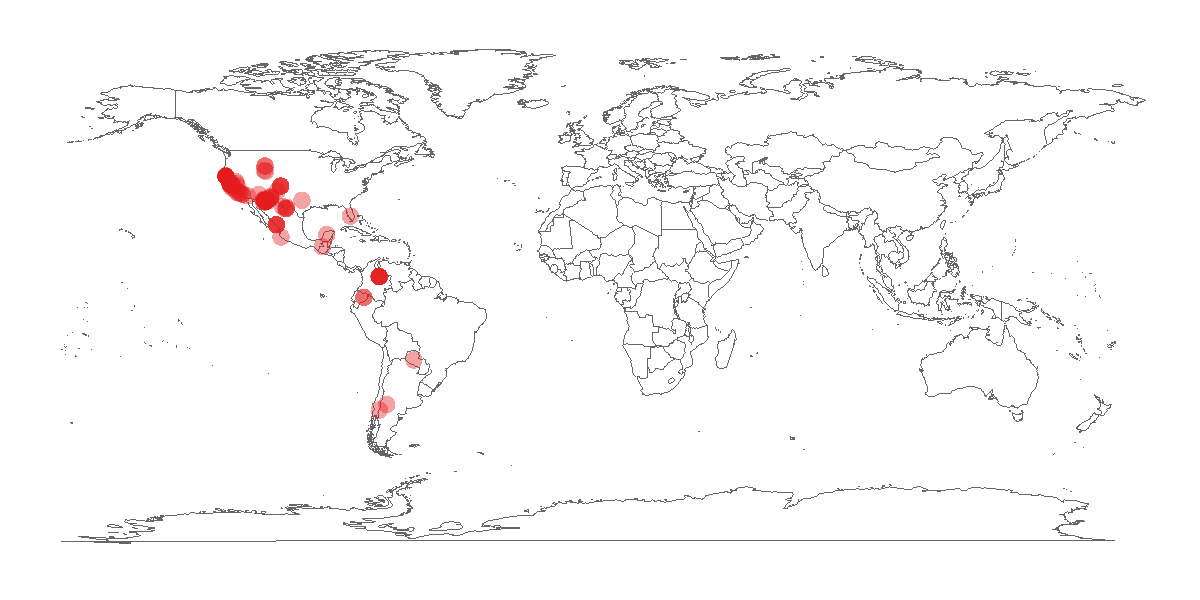
\includegraphics{components/figure/manuscript-unnamed-chunk-20-1.pdf}
\caption{}
\end{figure}

Another package, \href{https://github.com/ropensci/spocc}{spoccutils}

\subsection{GBIF data in other R
packages}\label{gbif-data-in-other-r-packages}

We discuss usage of GBIF data in other R packages throughout the
manuscript, but provide a synopsis here for clarity.

\subsubsection{taxize}\label{taxize}

Some of the GBIF taxonomic services are also avialable in
\href{https://github.com/ropensci/taxize}{taxize}, an R package that
focuses on getting data from taxonomic data sources on the web. For
example, with \texttt{get\_gbifid()} one can get GBIF IDs used for a set
of taxonomic names - then use those IDs in other functions in
\texttt{taxize} to get additional information, like taxonomically
downstream children.

\subsubsection{spocc}\label{spocc}

GBIF occurrence data is available in the R package
\href{https://github.com/ropensci/spocc}{spocc} via \texttt{rgbif}.
\texttt{spocc} is a unified interface for fetching species occurrence
data from many sources on the web. For example, a user can collect
occurrence data from GBIF, iDigBio, and iNaturalist, and easily combine
them, then use other pacakages to clean and vizualize the data.

\section{Use cases}\label{use-cases}

The following are three use cases for \texttt{rgbif}: niche modelling,
spatial change in biodiversity, and distribution mapping.

\subsubsection{Ecological niche
modelling}\label{ecological-niche-modelling}

In this example, we plot actual occurrence data for \emph{Bradypus}
species against a single predictor variable, BIO1 (annual mean
temperature). This is only ont step in a species distribution modelling
nworkflow.

This example can be done using BISON data as well with our rbison
package.

\emph{Load libraries}

\begin{Shaded}
\begin{Highlighting}[]
\KeywordTok{library}\NormalTok{(}\StringTok{"rgbif"}\NormalTok{)}
\KeywordTok{library}\NormalTok{(}\StringTok{"dismo"}\NormalTok{)}
\KeywordTok{library}\NormalTok{(}\StringTok{"maptools"}\NormalTok{)}
\KeywordTok{library}\NormalTok{(}\StringTok{"plyr"}\NormalTok{)}
\end{Highlighting}
\end{Shaded}

\emph{Raster files}

Make a list of files that are installed with the dismo package, then
create a rasterStack from these

\begin{Shaded}
\begin{Highlighting}[]
\NormalTok{files <-}\StringTok{ }\KeywordTok{list.files}\NormalTok{(}\KeywordTok{paste}\NormalTok{(}\KeywordTok{system.file}\NormalTok{(}\DataTypeTok{package =} \StringTok{"dismo"}\NormalTok{), }\StringTok{"/ex"}\NormalTok{, }\DataTypeTok{sep =} \StringTok{""}\NormalTok{),}
                    \StringTok{"grd"}\NormalTok{, }\DataTypeTok{full.names =} \OtherTok{TRUE}\NormalTok{)}
\NormalTok{predictors <-}\StringTok{ }\KeywordTok{stack}\NormalTok{(files)}
\end{Highlighting}
\end{Shaded}

\emph{Get world boundaries}

\begin{Shaded}
\begin{Highlighting}[]
\KeywordTok{data}\NormalTok{(wrld_simpl)}
\end{Highlighting}
\end{Shaded}

\emph{Get GBIF data using the rOpenSci package rgbif}

\begin{Shaded}
\begin{Highlighting}[]
\NormalTok{nn <-}\StringTok{ }\KeywordTok{name_lookup}\NormalTok{(}\StringTok{"bradypus*"}\NormalTok{, }\DataTypeTok{rank =} \StringTok{"species"}\NormalTok{)}
\NormalTok{nn <-}\StringTok{ }\KeywordTok{na.omit}\NormalTok{(}\KeywordTok{unique}\NormalTok{(nn$data$nubKey))}
\NormalTok{df <-}\StringTok{ }\KeywordTok{occ_search}\NormalTok{(}\DataTypeTok{taxonKey =} \NormalTok{nn, }\DataTypeTok{hasCoordinate =} \OtherTok{TRUE}\NormalTok{, }\DataTypeTok{limit =} \DecValTok{500}\NormalTok{)}
\NormalTok{df <-}\StringTok{ }\NormalTok{df[ }\KeywordTok{sapply}\NormalTok{(df, function(x) }\KeywordTok{class}\NormalTok{(x$data)) %in%}\StringTok{ "data.frame"} \NormalTok{]}
\NormalTok{df <-}\StringTok{ }\KeywordTok{ldply}\NormalTok{(}\KeywordTok{lapply}\NormalTok{(df, }\StringTok{"[["}\NormalTok{, }\StringTok{"data"}\NormalTok{))}
\NormalTok{df2 <-}\StringTok{ }\NormalTok{df[,}\KeywordTok{c}\NormalTok{(}\StringTok{'decimalLongitude'}\NormalTok{,}\StringTok{'decimalLatitude'}\NormalTok{)]}
\end{Highlighting}
\end{Shaded}

\emph{Plot}

\begin{enumerate}
\def\labelenumi{(\arabic{enumi})}
\itemsep1pt\parskip0pt\parsep0pt
\item
  Add raster data, (2) Add political boundaries, (3) Add the points
  (occurrences)
\end{enumerate}

\begin{Shaded}
\begin{Highlighting}[]
\KeywordTok{plot}\NormalTok{(predictors, }\DecValTok{1}\NormalTok{)}
\KeywordTok{plot}\NormalTok{(wrld_simpl, }\DataTypeTok{add =} \OtherTok{TRUE}\NormalTok{)}
\KeywordTok{points}\NormalTok{(df2, }\DataTypeTok{col =} \StringTok{"blue"}\NormalTok{)}
\end{Highlighting}
\end{Shaded}

\begin{figure}[htbp]
\centering
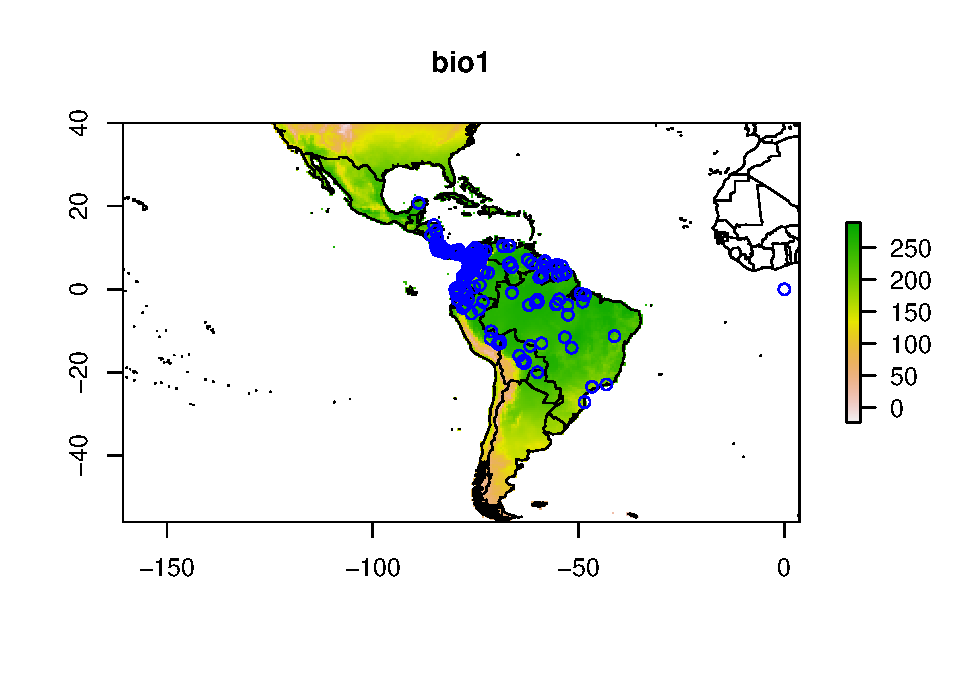
\includegraphics{components/figure/manuscript-unnamed-chunk-26-1.pdf}
\caption{}
\end{figure}

\subsubsection{Biodiversity in big
cities}\label{biodiversity-in-big-cities}

In this example, we collect specimen records across different cities
using GBIF data from the \texttt{rgbif} package.

\emph{Load libraries}

\begin{Shaded}
\begin{Highlighting}[]
\KeywordTok{library}\NormalTok{(}\StringTok{"rgbif"}\NormalTok{)}
\KeywordTok{library}\NormalTok{(}\StringTok{"ggplot2"}\NormalTok{)}
\KeywordTok{library}\NormalTok{(}\StringTok{"plyr"}\NormalTok{)}
\KeywordTok{library}\NormalTok{(}\StringTok{"RCurl"}\NormalTok{)}
\KeywordTok{library}\NormalTok{(}\StringTok{"RColorBrewer"}\NormalTok{)}
\end{Highlighting}
\end{Shaded}

\emph{Get bounding boxes for some cites}

Bounding lat/long data is from
\href{https://raw.github.com/amyxzhang/boundingbox-cities/master/boundbox.txt}{here}.

\begin{Shaded}
\begin{Highlighting}[]
\NormalTok{rawdat <-}\StringTok{ }\KeywordTok{getURL}\NormalTok{(}\StringTok{'https://raw.githubusercontent.com/amyxzhang/boundingbox-cities/master/boundbox.txt'}\NormalTok{)}
\NormalTok{dat <-}\StringTok{ }\KeywordTok{read.table}\NormalTok{(}\DataTypeTok{text =} \NormalTok{rawdat, }\DataTypeTok{header =} \OtherTok{FALSE}\NormalTok{, }\DataTypeTok{sep=}\StringTok{"}\CharTok{\textbackslash{}t}\StringTok{"}\NormalTok{, }\DataTypeTok{col.names=}\KeywordTok{c}\NormalTok{(}\StringTok{"city"}\NormalTok{,}\StringTok{"minlat"}\NormalTok{,}\StringTok{"maxlon"}\NormalTok{,}\StringTok{"maxlat"}\NormalTok{,}\StringTok{"minlon"}\NormalTok{))}
\NormalTok{dat <-}\StringTok{ }\KeywordTok{data.frame}\NormalTok{(}\DataTypeTok{city=}\NormalTok{dat$city, }\DataTypeTok{minlon=}\NormalTok{dat$minlon, }\DataTypeTok{minlat=}\NormalTok{dat$minlat, }\DataTypeTok{maxlon=}\NormalTok{dat$maxlon, }\DataTypeTok{maxlat=}\NormalTok{dat$maxlat)}
\end{Highlighting}
\end{Shaded}

\begin{Shaded}
\begin{Highlighting}[]
\NormalTok{getdata <-}\StringTok{ }\NormalTok{function(x)\{}
  \NormalTok{coords <-}\StringTok{ }\KeywordTok{as.numeric}\NormalTok{(x[}\KeywordTok{c}\NormalTok{(}\StringTok{'minlon'}\NormalTok{,}\StringTok{'minlat'}\NormalTok{,}\StringTok{'maxlon'}\NormalTok{,}\StringTok{'maxlat'}\NormalTok{)])}
  \NormalTok{num <-}\StringTok{ }\KeywordTok{occ_search}\NormalTok{(}\DataTypeTok{geometry =} \NormalTok{coords)$meta$count}
  \KeywordTok{data.frame}\NormalTok{(}\DataTypeTok{city=}\NormalTok{x[}\StringTok{'city'}\NormalTok{], }\DataTypeTok{richness=}\NormalTok{num, }\DataTypeTok{stringsAsFactors =} \OtherTok{FALSE}\NormalTok{)}
\NormalTok{\}}
\end{Highlighting}
\end{Shaded}

\begin{Shaded}
\begin{Highlighting}[]
\NormalTok{out <-}\StringTok{ }\KeywordTok{apply}\NormalTok{(dat, }\DecValTok{1}\NormalTok{, getdata)}
\end{Highlighting}
\end{Shaded}

\emph{Merge to original table}

\begin{Shaded}
\begin{Highlighting}[]
\NormalTok{out <-}\StringTok{ }\KeywordTok{merge}\NormalTok{(dat, }\KeywordTok{ldply}\NormalTok{(out), }\DataTypeTok{by=}\StringTok{"city"}\NormalTok{)}
\end{Highlighting}
\end{Shaded}

\emph{Add centroids from bounding boxes}

\begin{Shaded}
\begin{Highlighting}[]
\NormalTok{out <-}\StringTok{ }\KeywordTok{transform}\NormalTok{(out, }\DataTypeTok{lat =} \NormalTok{(minlat+maxlat)/}\DecValTok{2}\NormalTok{, }\DataTypeTok{lon =} \NormalTok{(minlon+maxlon)/}\DecValTok{2}\NormalTok{)}
\end{Highlighting}
\end{Shaded}

\emph{Plot data}

\begin{Shaded}
\begin{Highlighting}[]
\NormalTok{mapp <-}\StringTok{ }\KeywordTok{map_data}\NormalTok{(}\StringTok{'world'}\NormalTok{)}
\KeywordTok{ggplot}\NormalTok{(mapp, }\KeywordTok{aes}\NormalTok{(long, lat)) +}
\StringTok{  }\KeywordTok{geom_polygon}\NormalTok{(}\KeywordTok{aes}\NormalTok{(}\DataTypeTok{group=}\NormalTok{group), }\DataTypeTok{fill=}\StringTok{"white"}\NormalTok{, }\DataTypeTok{alpha=}\DecValTok{0}\NormalTok{, }\DataTypeTok{color=}\StringTok{"black"}\NormalTok{, }\DataTypeTok{size=}\FloatTok{0.4}\NormalTok{) +}
\StringTok{  }\KeywordTok{geom_point}\NormalTok{(}\DataTypeTok{data=}\NormalTok{out, }\KeywordTok{aes}\NormalTok{(lon, lat, }\DataTypeTok{color=}\NormalTok{richness), }\DataTypeTok{size=}\DecValTok{5}\NormalTok{, }\DataTypeTok{alpha=}\FloatTok{0.8}\NormalTok{) +}
\StringTok{  }\KeywordTok{scale_color_continuous}\NormalTok{(}\DataTypeTok{low =} \StringTok{"#60E1EE"}\NormalTok{, }\DataTypeTok{high =} \StringTok{"#0404C8"}\NormalTok{) +}
\StringTok{  }\KeywordTok{labs}\NormalTok{(}\DataTypeTok{x=}\StringTok{""}\NormalTok{, }\DataTypeTok{y=}\StringTok{""}\NormalTok{) +}
\StringTok{  }\KeywordTok{theme_grey}\NormalTok{(}\DataTypeTok{base_size=}\DecValTok{14}\NormalTok{) +}
\StringTok{  }\KeywordTok{theme}\NormalTok{(}\DataTypeTok{legend.position =} \StringTok{"bottom"}\NormalTok{, }\DataTypeTok{legend.key =} \KeywordTok{element_blank}\NormalTok{()) +}
\StringTok{  }\KeywordTok{guides}\NormalTok{(}\DataTypeTok{color =} \KeywordTok{guide_legend}\NormalTok{(}\DataTypeTok{keywidth =} \DecValTok{2}\NormalTok{))}
\end{Highlighting}
\end{Shaded}

\begin{figure}[htbp]
\centering
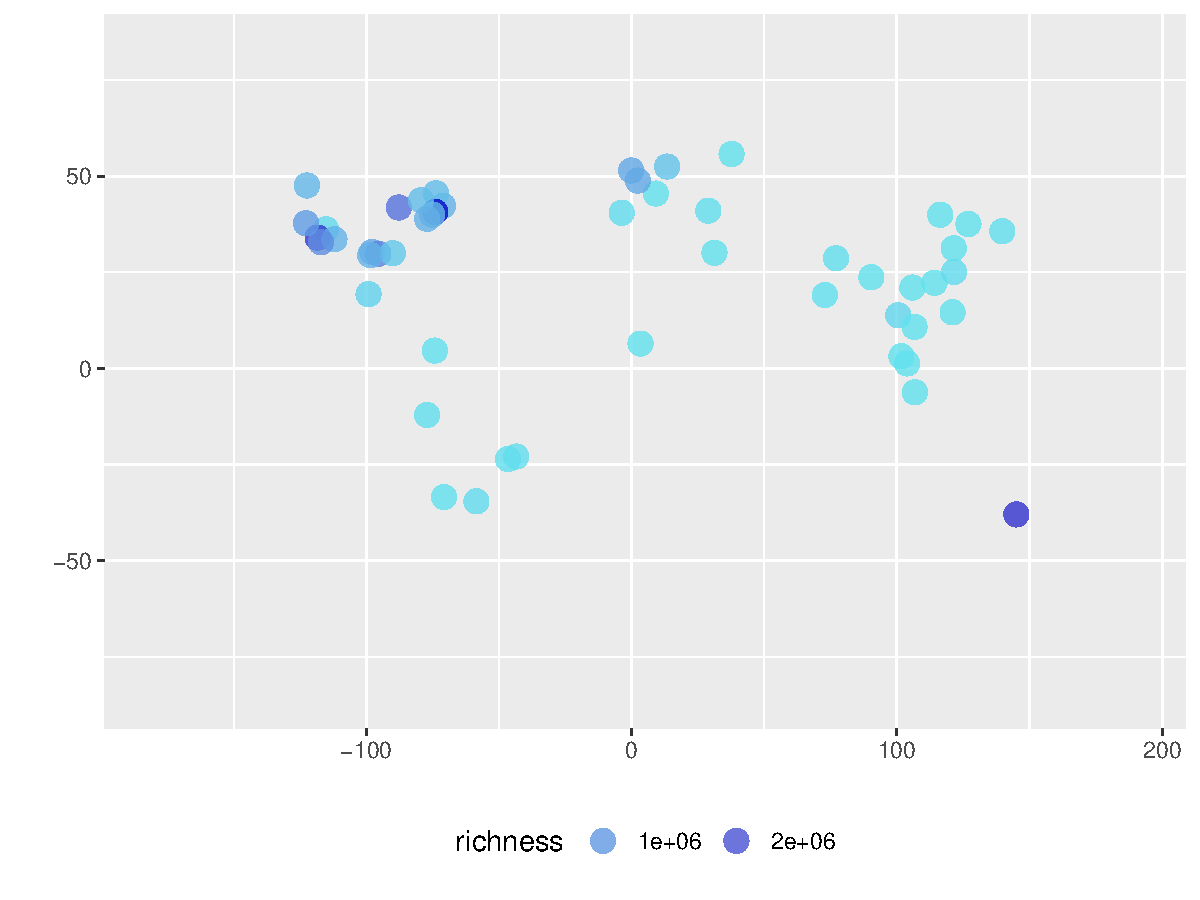
\includegraphics{components/figure/manuscript-unnamed-chunk-31-1.pdf}
\caption{}
\end{figure}

\subsubsection{Valley oak occurrence data
comparison}\label{valley-oak-occurrence-data-comparison}

This example comes from \href{https://twitter.com/ajpelu}{Antonio J.
Perez-Luque} who
\href{https://twitter.com/ajpelu/status/473951167567757312}{shared his
plot on Twitter}. Antonio compared the occurrences of Valley Oak
(\emph{Quercus lobata}) from \href{http://www.gbif.org/}{GBIF} to the
distribution of the same species from the
\href{http://esp.cr.usgs.gov/data/little/}{Atlas of US Trees}.

\emph{Load libraries}

\begin{Shaded}
\begin{Highlighting}[]
\KeywordTok{library}\NormalTok{(}\StringTok{'rgbif'}\NormalTok{)}
\KeywordTok{library}\NormalTok{(}\StringTok{'raster'}\NormalTok{)}
\KeywordTok{library}\NormalTok{(}\StringTok{'sp'}\NormalTok{)}
\KeywordTok{library}\NormalTok{(}\StringTok{'maptools'}\NormalTok{)}
\KeywordTok{library}\NormalTok{(}\StringTok{'rgeos'}\NormalTok{)}
\KeywordTok{library}\NormalTok{(}\StringTok{'scales'}\NormalTok{)}
\end{Highlighting}
\end{Shaded}

\emph{Get GBIF Data for Quercus lobata}

\begin{Shaded}
\begin{Highlighting}[]
\NormalTok{keyQl <-}\StringTok{ }\KeywordTok{name_backbone}\NormalTok{(}\DataTypeTok{name=}\StringTok{'Quercus lobata'}\NormalTok{, }\DataTypeTok{kingdom=}\StringTok{'plants'}\NormalTok{)$speciesKey}
\NormalTok{dat.Ql <-}\StringTok{ }\KeywordTok{occ_search}\NormalTok{(}\DataTypeTok{taxonKey=}\NormalTok{keyQl, }\DataTypeTok{return=}\StringTok{'data'}\NormalTok{, }\DataTypeTok{limit=}\DecValTok{50000}\NormalTok{)}
\end{Highlighting}
\end{Shaded}

\emph{Get Distribution map of Q. lobata Atlas of US Trees (Little, E.)}

From
\href{http://esp.cr.usgs.gov/data/little/}{\url{http://esp.cr.usgs.gov/data/little/}}.
And save shapefile in same directory

\begin{Shaded}
\begin{Highlighting}[]
\NormalTok{url <-}\StringTok{ 'http://esp.cr.usgs.gov/data/little/querloba.zip'}
\NormalTok{tmp <-}\StringTok{ }\KeywordTok{tempdir}\NormalTok{()}
\KeywordTok{download.file}\NormalTok{(url, }\DataTypeTok{destfile =} \StringTok{"~/querloba.zip"}\NormalTok{)}
\KeywordTok{unzip}\NormalTok{(}\StringTok{"~/querloba.zip"}\NormalTok{, }\DataTypeTok{exdir =} \NormalTok{tmp)}
\NormalTok{ql <-}\StringTok{ }\KeywordTok{readShapePoly}\NormalTok{(}\KeywordTok{file.path}\NormalTok{(tmp, }\StringTok{"querloba.shp"}\NormalTok{))}
\end{Highlighting}
\end{Shaded}

\emph{Get Elevation data of US}

\begin{Shaded}
\begin{Highlighting}[]
\NormalTok{alt.USA <-}\StringTok{ }\KeywordTok{getData}\NormalTok{(}\StringTok{'alt'}\NormalTok{, }\DataTypeTok{country =} \StringTok{'USA'}\NormalTok{)}
\end{Highlighting}
\end{Shaded}

\emph{Create Hillshade of US}

\begin{Shaded}
\begin{Highlighting}[]
\NormalTok{alt.USA <-}\StringTok{ }\NormalTok{alt.USA[[}\DecValTok{1}\NormalTok{]]}
\NormalTok{slope.USA <-}\StringTok{ }\KeywordTok{terrain}\NormalTok{(alt.USA, }\DataTypeTok{opt =} \StringTok{'slope'}\NormalTok{)}
\NormalTok{aspect.USA <-}\StringTok{ }\KeywordTok{terrain}\NormalTok{(alt.USA, }\DataTypeTok{opt =} \StringTok{'aspect'}\NormalTok{)}
\NormalTok{hill.USA <-}\StringTok{ }\KeywordTok{hillShade}\NormalTok{(slope.USA, aspect.USA, }\DataTypeTok{angle =} \DecValTok{45}\NormalTok{, }\DataTypeTok{direction =} \DecValTok{315}\NormalTok{)}
\end{Highlighting}
\end{Shaded}

\emph{Plot map}

\begin{Shaded}
\begin{Highlighting}[]
\KeywordTok{plot}\NormalTok{(hill.USA, }\DataTypeTok{col =} \KeywordTok{grey}\NormalTok{(}\DecValTok{0}\NormalTok{:}\DecValTok{100}\NormalTok{/}\DecValTok{100}\NormalTok{), }\DataTypeTok{legend =} \OtherTok{FALSE}\NormalTok{, }\DataTypeTok{xlim =} \KeywordTok{c}\NormalTok{(-}\DecValTok{125}\NormalTok{, -}\DecValTok{116}\NormalTok{), }\DataTypeTok{ylim =} \KeywordTok{c}\NormalTok{(}\DecValTok{32}\NormalTok{, }\DecValTok{42}\NormalTok{), }\DataTypeTok{main =} \StringTok{'Distribution of Quercus lobata'}\NormalTok{, }\DataTypeTok{xlab =} \StringTok{"Long"}\NormalTok{, }\DataTypeTok{ylab =} \StringTok{'Lat'}\NormalTok{)}
\CommentTok{# add shape from Atlas of US Trees}
\KeywordTok{plot}\NormalTok{(ql, }\DataTypeTok{add =} \OtherTok{TRUE}\NormalTok{, }\DataTypeTok{col =} \KeywordTok{alpha}\NormalTok{(}\StringTok{"white"}\NormalTok{, }\FloatTok{0.6}\NormalTok{), }\DataTypeTok{border =} \OtherTok{FALSE}\NormalTok{)}
\CommentTok{# add Gbif presence points}
\KeywordTok{points}\NormalTok{(dat.Ql$decimalLongitude, dat.Ql$decimalLatitude, }\DataTypeTok{cex =} \NormalTok{.}\DecValTok{7}\NormalTok{, }\DataTypeTok{pch =} \DecValTok{19}\NormalTok{, }\DataTypeTok{col =} \KeywordTok{alpha}\NormalTok{(}\StringTok{"darkgreen"}\NormalTok{, }\FloatTok{0.8}\NormalTok{))}
\KeywordTok{legend}\NormalTok{(}\DataTypeTok{x =} \NormalTok{-}\DecValTok{121}\NormalTok{, }\DataTypeTok{y =} \FloatTok{40.5}\NormalTok{, }\StringTok{"GBIF Data"}\NormalTok{, }\DataTypeTok{pch =} \DecValTok{19}\NormalTok{, }\DataTypeTok{col =} \StringTok{'darkgreen'}\NormalTok{, }\DataTypeTok{bty =} \StringTok{'n'}\NormalTok{, }\DataTypeTok{pt.cex =} \DecValTok{1}\NormalTok{, }\DataTypeTok{cex =} \NormalTok{.}\DecValTok{8}\NormalTok{)}
\KeywordTok{legend}\NormalTok{(}\DataTypeTok{x =} \NormalTok{-}\DecValTok{121}\NormalTok{, }\DataTypeTok{y =} \FloatTok{41.5}\NormalTok{, }\StringTok{"Atlas of United States Trees }\CharTok{\textbackslash{}n}\StringTok{ (Little, E. 1971)"}\NormalTok{, }\DataTypeTok{pt.cex =} \FloatTok{1.5}\NormalTok{, }\DataTypeTok{cex =} \NormalTok{.}\DecValTok{8}\NormalTok{, }\DataTypeTok{pch =} \DecValTok{19}\NormalTok{, }\DataTypeTok{col =} \StringTok{'white'}\NormalTok{, }\DataTypeTok{bty =} \StringTok{'n'}\NormalTok{)}
\end{Highlighting}
\end{Shaded}

\begin{figure}[htbp]
\centering
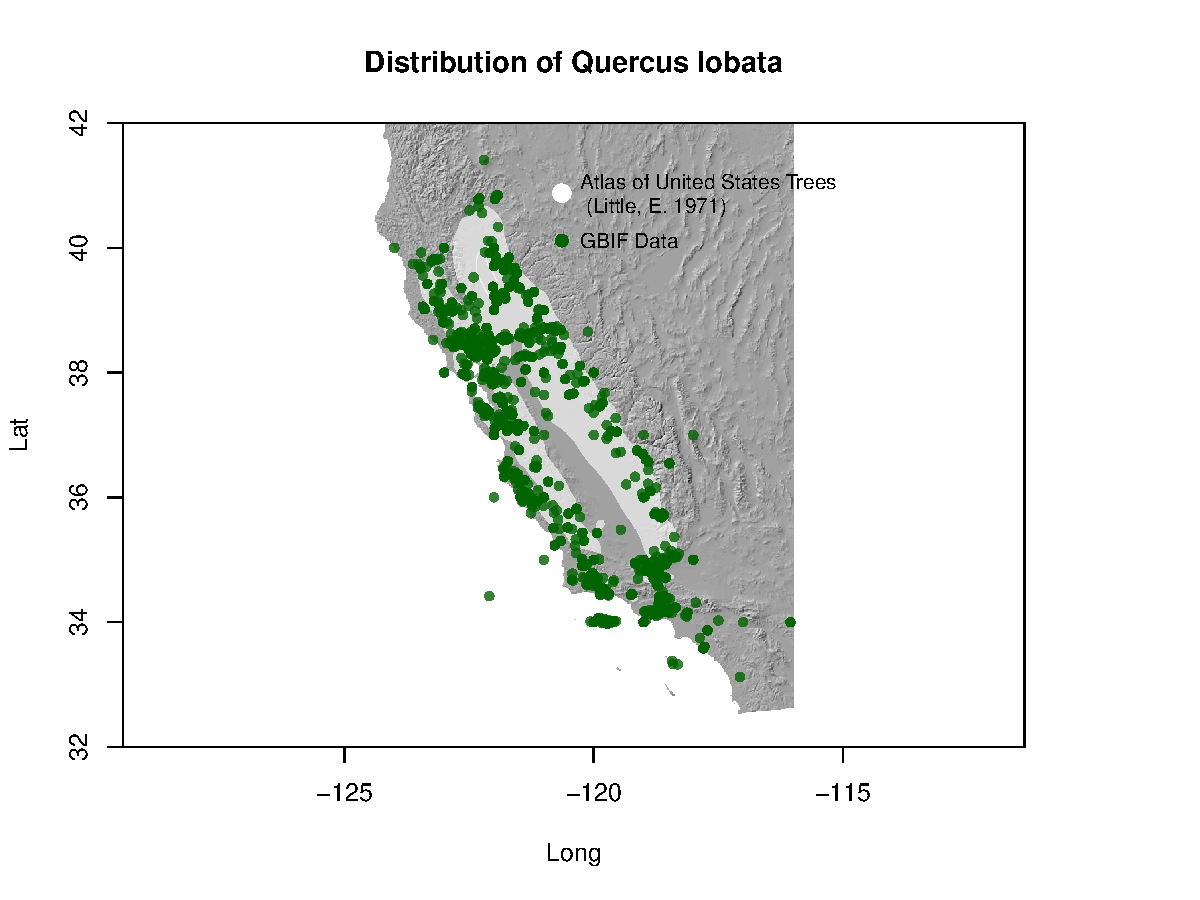
\includegraphics{components/figure/manuscript-unnamed-chunk-38-1.pdf}
\caption{}
\end{figure}

\section{Conclusions and future
directions}\label{conclusions-and-future-directions}

The \texttt{rgbif} R package provides a programmatic interface to GBIF's
application programming interface (API) - a powerful tool for making
research using species occurrence data reproducible. In fact, the
\texttt{rgbif} package has already been used in 22 scholarly
publications (as of 2015-11-14).

The \texttt{rgbif} package is relatively stable, and should not have
many breaking changes unless necessitated due to changes in the GBIF
API.

One area of focus in the future is to attempt to solve many use cases
that have been brought up with respect to GBIF data. For example, some
specimens are included in GBIF that are located in botanical gardens.
For many research questions, researchers are interested in ``wild'' type
occurrences, not those in human curated scenarios. Making removal of
these occurrences easy would be very useful, but is actually quite a
hard problem.

\section{Acknowledgements}\label{acknowledgements}

This project was supported in part by the Alfred P Sloan Foundation
(Grant 2013-6-22), and the Helmsley Foundation (Grant XXXXXX).

\section{Data Accessibility}\label{data-accessibility}

All scripts and data used in this paper can be found in the permanent
data archive Zenodo under the digital object identifier (DOI). This DOI
corresponds to a snapshot of the GitHub repository at
\href{https://github.com/sckott/msrgbif}{github.com/sckott/msrgbif}.
Software can be found at
\href{https://github.com/ropensci/rgbif}{\url{https://github.com/ropensci/rgbif}},
under an MIT license.

\section*{References}\label{references}
\addcontentsline{toc}{section}{References}

Beck J., Ballesteros-Mejia L., Buchmann CM., Dengler J., Fritz SA.,
Gruber B., Hof C., Jansen F., Knapp S., Kreft H., Schneider A-K., Winter
M., Dormann CF. 2012. Whats on the horizon for macroecology?
\emph{Ecography} 35:673--683.

Brown JH. 1995. \emph{Macroecology}. University of Chicago Press.

Brown KA., Parks KE., Bethell CA., Johnson SE., Mulligan M. 2015.
Predicting plant diversity patterns in madagascar: Understanding the
effects of climate and land cover change in a biodiversity hotspot.
\emph{PLOS ONE} 10:e0122721.

Ceballos G., Ehrlich PR., Barnosky AD., Garcia A., Pringle RM., Palmer
TM. 2015. Accelerated modern human-induced species losses: Entering the
sixth mass extinction. \emph{Science Advances} 1:e1400253--e1400253.

Chamberlain S., Ram K., Barve V., Mcglinn D. \emph{Rgbif: Interface to
the global 'biodiversity' information facility 'aPI'}.

Faulkner KT., Robertson MP., Rouget M., Wilson JR. 2014. A simple, rapid
methodology for developing invasive species watch lists.
\emph{Biological Conservation} 179:25--32.

Febbraro MD., Lurz PWW., Genovesi P., Maiorano L., Girardello M.,
Bertolino S. 2013. The use of climatic niches in screening procedures
for introduced species to evaluate risk of spread: A case with the
american eastern grey squirrel. \emph{PLoS ONE} 8:e66559.

Ferretti F., Verd GM., Seret B., {Š}prem JS., Micheli F. 2015. Falling
through the cracks: The fading history of a large iconic predator.
\emph{Fish and Fisheries}:n/a--n/a.

Ficetola GF., Rondinini C., Bonardi A., Baisero D., Padoa-Schioppa E.
2014. Habitat availability for amphibians and extinction threat: A
global analysis. \emph{Diversity and Distributions} 21:302--311.

Mar{í}a Mendoza., Ospina OE., C{á}rdenas-Henao H., Garc{í}a-R JC. 2015.
A likelihood inference of historical biogeography in the world's most
diverse terrestrial vertebrate genus: Diversification of
direct-developing frogs (craugastoridae: Pristimantis) across the
neotropics. \emph{Molecular Phylogenetics and Evolution} 85:50--58.

Pimm SL., Jenkins CN., Abell R., Brooks TM., Gittleman JL., Joppa LN.,
Raven PH., Roberts CM., Sexton JO. 2014. The biodiversity of species and
their rates of extinction, distribution, and protection. \emph{Science}
344:1246752--1246752.

R Core Team. 2014. \emph{R: A language and environment for statistical
computing}. Vienna, Austria: R Foundation for Statistical Computing.

\end{document}


